\documentclass[a4paper,12pt]{article}

\usepackage[utf8]{inputenc}
\usepackage[T1]{fontenc}
\usepackage[a4paper,total={150mm,240mm}]{geometry}
\usepackage{amsmath}
\usepackage{amsfonts}
\usepackage{amsthm}
\usepackage{amscd}
\usepackage{grffile}
\usepackage{tikz}
\usepackage{eurosym}
\usepackage{graphicx}
\usepackage{color}
\usepackage{listings}
\lstset{language=C++, basicstyle=\ttfamily,
  keywordstyle=\color{black}\bfseries, tabsize=4, stringstyle=\ttfamily,
  commentstyle=\itshape, extendedchars=true, escapeinside={/*@}{@*/}}
\usepackage{paralist}
\usepackage{curves}
\usepackage{calc}
\usepackage{picinpar}
\usepackage{enumerate}
\usepackage{algpseudocode}
\usepackage{bm}
\usepackage{multibib}
\usepackage{hyperref}
\usepackage{textcase}
\usepackage{nicefrac}

\definecolor{listingbg}{gray}{0.95}

\title{DUNE PDELab Tutorial 04 \\
Finite Elements for the Wave Equation}
\author{DUNE/PDELab Team}
\date{\today}

\begin{document}

\maketitle
\tableofcontents
\clearpage

\section{Introduction}

In this tutorial we solve the wave equation formulated as a first order
in time system. This way the example serves as a model for the
treatment of systems of partial differential equations in PDELab.

\subsection*{Depends On} This tutorial depends on tutorial 01 and 03.

\section{PDE Problem}

As an example for a system we consider the wave equation with reflective boundary conditions:
\begin{subequations}
\label{eq:WaveEquation}
\begin{align}
\partial_{tt} u-c^2\Delta u  &= 0 &&\text{in $\Omega\times\Sigma$},\\
u &= 0 &&\text{on $\partial\Omega$},\\
u &= q &&\text{at $t=0$},\\
\partial_t u &= w &&\text{at $t=0$},
\end{align}
\end{subequations}
where $c$ is the speed of sound.
Renaming $u_0=u$ and introducing $u_1=\partial_t u_0 =\partial_t u$ we can write the wave equation as a system of two equations:
\begin{subequations}
\label{eq:SystemForm1}
\begin{align}
\partial_t u_1 - c^2\Delta u_0 &=0 &&\text{in $\Omega\times\Sigma$}, \label{eq:2a}\\
\partial_t u_0 - u_1 &=0 &&\text{in $\Omega\times\Sigma$}, \label{eq:2b}\\
u_0 &= 0 &&\text{on $\partial\Omega$},\\
u_1 &= 0 &&\text{on $\partial\Omega$},\\
u_0 &= q &&\text{at $t=0$},\\
u_1 &= w &&\text{at $t=0$}.
\end{align}
\end{subequations}
Since $u_0=u=0$ on the boundary we also have $\partial_t u = u_1 = 0$ on the boundary.
But one may also omit the boundary condition on $u_1$.

Note that there are several alternative ways how to write the scalar equation
\eqref{eq:WaveEquation} as a system of PDEs:
\begin{itemize}
\item Eriksson et al. in \cite{Eriksson} apply the Laplacian to
equation \eqref{eq:2b}
\begin{equation}
\Delta \partial_t u_0 - \Delta u_1 = 0
\end{equation} \label{eq:Eriksson}
which has advantages for energy conservation but requires additional smoothness
properties.
\item Alternatively, we may introduce the abbreviations
$q=\partial_t u$ and $w=-\nabla u$, so $\partial_{tt} u - c^2 \Delta u =
\partial_{tt} u - c^2 \nabla\cdot\nabla u = \partial_{t} q + c^2 \nabla\cdot w = 0$.
Taking partial derivatives of the introduced variables we obtain $\partial_{x_i} q=
\partial_{x_i} \partial_t u = \partial_t \partial_{x_i}  u = - \partial_t w_i$. This results
in a first-order hyperbolic system of PDEs for $q$ and $w$
\begin{align*}
\partial_t q + c^2 \nabla\cdot w &= 0\\
\partial_t w + \nabla q &= 0
\end{align*}
which are called equations of linear acoustics \cite{LeVeque}. This formulation
is physically more relevant. It can be modified to handle discontinuous material
properties and upwind finite volume methods can be used for numerical treatment.
\end{itemize}

Here we will stay, however, with the simplest formulation \eqref{eq:SystemForm1}
for simplicity.

\subsection*{Weak Formulation}

Multiplying \eqref{eq:2a}
with the test function $v_0$ and \eqref{eq:2b} with the test function $v_1$
and using integration by parts we arrive at the weak formulation: Find $(u_0(t),u_1(t))\in
U_0\times U_1$ s.t.
\begin{align}
  d_t (u_1,v_0)_{0,\Omega} + c^2 (\nabla u_0, \nabla v_0)_{0,\Omega} &=
  0 \quad \forall v_0 \in U_0 \notag \\
  d_t (u_0,v_1)_{0,\Omega} - (u_1,v_1)_{0,\Omega} &= 0 \quad \forall
  v_1 \in U_1 \label{eq:WeakFormSystem}
\end{align}
where we used the notation of the $L^2$ inner product $(u,v)_{0,\Omega} = \int_\Omega
u v \, dx$. An equivalent formulation to (\ref{eq:WeakFormSystem}) that
hides the system structure reads as follows:
\begin{equation}
\label{eq:WeakForm}
\begin{split}
d_t &\left[ (u_0,v_1)_{0,\Omega} + (u_1,v_0)_{0,\Omega}\right] \\
&\hspace{20mm}+ \left[ c^2 (\nabla u_0,\nabla v_0)_{0,\Omega} -(u_1,v_1)_{0,\Omega} \right] = 0
\quad \forall (v_0,v_1)\in U_0\times U_1
\end{split}
\end{equation}
With the latter we readily identify the temporal and spatial residual
forms:
\begin{align}
m^{\text{WAVE}}((u_0,u_1),(v_0,v_1)) &= (u_0,v_1)_{0,\Omega} + (u_1,v_0)_{0,\Omega},
\label{eq:TemporalResForm}\\
r^{\text{WAVE}}((u_0,u_1),(v_0,v_1)) &= c^2 (\nabla u_0,\nabla
v_0)_{0,\Omega} - (u_1,v_1)_{0,\Omega} \; , \label{eq:SpatialResForm}
\end{align}
while with the former the system structure is more visible which might
help to understand the implementation presented in section
\ref{sec:funct-driver}.
The spaces $U_0$ and $U_1$ can differ as different types of boundary
conditions can be incorporated into the ansatz spaces. But here both
spaces are constrained by homogeneous Dirichlet boundary conditions.

\subsection*{Generalization}

The abstract setting of PDELab with its weighted residual formulation
carries over to the case of systems of
partial differential equations when cartesian products of
functions spaces are introduced, i.e. the abstract \textit{stationary} problem then reads
\begin{equation}
\text{Find $u_h\in U_h=U_h^1\times \ldots \times U_h^s$ s.t.:} \quad r_h(u_h,v)=0
\quad \forall v\in V_h=V_h^1\times\ldots\times V_h^s
\label{Eq:BasicSystemBuildingBlock}
\end{equation}
with $s$ the number of components in the system. Again the concepts
are completely orthogonal meaning that $r_h$ might be affine linear or nonlinear
in its first argument and the instationary case works as well.

From an organizational point of view it makes sense to allow that
a component space $U_h^i$ in the cartesian product is itself
a product space. This naturally leads to a \textit{tree structure} in the
function spaces.

Consider as an example the Stokes equation in $d$ space dimensions.
There one has pressure $p$ and velocity $v$ with components $v_1,\ldots,v_d$
as unknowns. An appropriate function space then would be
$$ U = (P,(V^1,\ldots,V^d)).$$

\section{Finite Element Method}

The finite element method applied to \eqref{eq:WeakForm} is straightforward.
We may use the conforming space $V_h^{k,d}(\mathcal{T}_h)$ of degree $k$
in dimension $d$ for each of the components. Typically one would choose
the same polynomial degree for both components.

\section{Realization in PDELab}

The structure of the code is very similar to that of tutorial 01 and 03.
It consists of the following files:
\begin{enumerate}[1)]
\item The ini-file
\lstinline{tutorial04.ini} holds parameters read by various parts of the code
which control the execution.
\item The main file \lstinline{tutorial04.cc} includes the necessary C++,
DUNE and PDELab header files
and contains the \lstinline{main} function where the execution starts.
The purpose of the \lstinline{main} function is
to instantiate DUNE grid objects and call the \lstinline{driver} function.
\item File \lstinline{driver.hh} instantiates the necessary PDELab classes
for solving a linear instationary problem and finally solves the problem.
\item File \lstinline{wavefem.hh} contains the local operator classes
\lstinline{WaveFEM} and \lstinline{WaveL2} realizing the spatial
and temporal residual forms.
\end{enumerate}

\subsection{Ini-File}

The ini-file contains the usual sections for structured and 1d grids. The
\lstinline{fem} section is the same as in tutorial 01 and allows to set
the polynomial degree, temporal integration order and the time step size.
The \lstinline{problem} section has a new parameter for the speed of sound.
\lstinputlisting[basicstyle=\ttfamily\small,
frame=single,
backgroundcolor=\color{listingbg}]{../src/tutorial04.ini}

\subsection{Function \lstinline{main}}

The \lstinline{main} function is very similar to the one in tutorial 03.
In order to simplify things only the structured grids \lstinline{OneDGrid}
and \lstinline{YaspGrid} are used.

\subsection{Function \lstinline{driver}}
\label{sec:funct-driver}

The \lstinline{driver} function gets a grid view, a finite element
map and a parameter tree and its purpose is to solve the problem on
the given mesh.
\lstinputlisting[linerange={6-8},
basicstyle=\ttfamily\small,
frame=single,
backgroundcolor=\color{listingbg}]{../src/driver.hh}

There are several changes now in the driver due to the system of PDEs.
The first step is to set up the grid function space using the given finite
element map:
\lstinputlisting[linerange={15-18},
basicstyle=\ttfamily\small,
frame=single,
backgroundcolor=\color{listingbg}]{../src/driver.hh}

The next step is to set up the product space containing
two components. This is done by the following code section:
\lstinputlisting[linerange={21-26},
basicstyle=\ttfamily\small,
frame=single,
backgroundcolor=\color{listingbg}]{../src/driver.hh}
PDELab offers two different class templates to build product spaces. The
one used here is \lstinline{PowerGridFunctionSpace} which creates
a product of a compile-time given number (2 here)
of \textit{identical} function spaces (\lstinline{GFS0} here)
which may only differ in the constraints. With the
class template \lstinline{CompositeGridFunctionSpace} you can create
a product space where all components might be different spaces.

An important aspect of product spaces is the ordering of the corresponding degrees
of freedom. Often the solvers need to exploit an underlying block structure
of the matrices.

This works in two stages: An ordering has first to be specified when creating product spaces
which is then subsequently exploited in the backend.
Here we use the \lstinline{EntityBlockedOrderingTag} to specify that all degrees of
freedom related to a geometric entity should be numbered consecutively in
the coefficient vector. Other options are the \lstinline{LexicographicOrderingTag}
ordering first all degrees of freedom of the first component space, then
all of the second component space and so on.
With the Iterative Solver Template Library ISTL it is now
possible to exploit the block structure at compile-time.
Here we use the tag \lstinline{fixed} in the ISTL vector backend to indicate
that at this level we want to create blocks of fixed size (in this case the block size will be two --
corresponding to the degrees of freedom per entity). Another option
would be the tag \lstinline{none} which is the default. Then the degrees
of freedom are still ordered in the specified way but no block structure is
introduced on the ISTL level. \textit{Important notice:} Using fixed block
structure in ISTL requires that there is the same number of degrees of freedom
per entity. This is true for polynomial degrees one and two but \textit{not}
for higher polynomial degree!

In order to define a function that specifies the initial value we can
use the same techniques as in the scalar case. We first define a lambda
closure
\lstinputlisting[linerange={29-34},
basicstyle=\ttfamily\small,
frame=single,
backgroundcolor=\color{listingbg}]{../src/driver.hh}
now returning two components in a \lstinline{FieldVector}.
The first component is the initial value for $u$ and the second component
is the initial value for $\partial_t u$. Then a PDELab grid function
can be constructed from the lambda closure
\lstinputlisting[linerange={35-35},
basicstyle=\ttfamily\small,
frame=single,
backgroundcolor=\color{listingbg}]{../src/driver.hh}

Using the grid function a coefficient vector can now be initialized:
\lstinputlisting[linerange={38-40},
basicstyle=\ttfamily\small,
frame=single,
backgroundcolor=\color{listingbg}]{../src/driver.hh}

Given a product function space it is also possible to
extract the individual component spaces from the product
space. This is done by the following code section:
\lstinputlisting[linerange={43-48},
basicstyle=\ttfamily\small,
frame=single,
backgroundcolor=\color{listingbg}]{../src/driver.hh}
In fact, one could have a tree-structured function space and
extract an arbitrary node as a function space.

The component spaces can now be used to build
up discrete grid functions for the two solution components:
\lstinputlisting[linerange={51-54},
basicstyle=\ttfamily\small,
frame=single,
backgroundcolor=\color{listingbg}]{../src/driver.hh}
Note that the full solution vector \lstinline{z} is passed as an argument.
The subspace automatically extracts the required components from the solution vector.

The next step is to assemble the constraints container for the composite
function space. Unfortunately there is currently no way to define the
constraints for both components in one go. We need to
set up a separate lambda closure for each component:
\lstinputlisting[linerange={57-62},
basicstyle=\ttfamily\small,
frame=single,
backgroundcolor=\color{listingbg}]{../src/driver.hh}
and then combine it using:
\lstinputlisting[linerange={63-65},
basicstyle=\ttfamily\small,
frame=single,
backgroundcolor=\color{listingbg}]{../src/driver.hh}
Note that you could define different constraints for each component
space although it is the same underlying function space.

Now the constraints container can be assembled as before:
\lstinputlisting[linerange={66-69},
basicstyle=\ttfamily\small,
frame=single,
backgroundcolor=\color{listingbg}]{../src/driver.hh}

The rest of the driver is the same as for tutorial 03 except that
a linear solver is used instead of Newton's method.

\subsection{Spatial Local Operator}

The spatial residual form \eqref{eq:SpatialResForm} is
implemented by the local operator \lstinline{WaveFEM} in
file \lstinline{wavefem.hh}. Cache construction and flags settings
are the same as in tutorial 01 and 03. Only volume terms are used here.
Note also that no parameter object is necessary as the only parameter
is the speed of sound $c$.

\subsubsection*{\lstinline{alpha_volume} method}

The method \lstinline{alpha_volume} has the \textit{same} interface
as in the scalar case:
\lstinputlisting[linerange={53-56},
basicstyle=\ttfamily\small,
frame=single,
backgroundcolor=\color{listingbg}]{../src/wavefem.hh}
However the trial and test function spaces \lstinline{LFSU} and \lstinline{LFSV}
now reflect the component structure of the global function space, i.e.
they consist of two components.

\textit{Important notice: Here we assume that trial and test space are identical
(up to constraints) and that also both components are identical!}

The two components can be extracted with the following code
\lstinputlisting[linerange={59-61},
basicstyle=\ttfamily\small,
frame=single,
backgroundcolor=\color{listingbg}]{../src/wavefem.hh}
The function spaces \lstinline{lfsu0} and \lstinline{lfsu1} are
now scalar spaces (which we assume to be identical).

After extracting the dimension
\lstinputlisting[linerange={64-64},
basicstyle=\ttfamily\small,
frame=single,
backgroundcolor=\color{listingbg}]{../src/wavefem.hh}
we select a quadrature rule
\lstinputlisting[linerange={67-69},
basicstyle=\ttfamily\small,
frame=single,
backgroundcolor=\color{listingbg}]{../src/wavefem.hh}
and may now loop over the quadrature points.

For each quadrature point, evaluate the basis function
of the first component:
\lstinputlisting[linerange={75-76},
basicstyle=\ttfamily\small,
frame=single,
backgroundcolor=\color{listingbg}]{../src/wavefem.hh}
As the components are identical we need only evaluate the basis once
and can compute the value of $u_1$ at the quadrature point
\lstinputlisting[linerange={79-81},
basicstyle=\ttfamily\small,
frame=single,
backgroundcolor=\color{listingbg}]{../src/wavefem.hh}
Then we evaluate the gradients of the basis functions
\lstinputlisting[linerange={84-85},
basicstyle=\ttfamily\small,
frame=single,
backgroundcolor=\color{listingbg}]{../src/wavefem.hh}
transform them from the reference element to the real element
\lstinputlisting[linerange={88-92},
basicstyle=\ttfamily\small,
frame=single,
backgroundcolor=\color{listingbg}]{../src/wavefem.hh}
and compute the gradient of $u_0$:
\lstinputlisting[linerange={95-97},
basicstyle=\ttfamily\small,
frame=single,
backgroundcolor=\color{listingbg}]{../src/wavefem.hh}
With the integration factor
\lstinputlisting[linerange={100-101},
basicstyle=\ttfamily\small,
frame=single,
backgroundcolor=\color{listingbg}]{../src/wavefem.hh}
the residuals can now be accumulated:
\lstinputlisting[linerange={102-105},
basicstyle=\ttfamily\small,
frame=single,
backgroundcolor=\color{listingbg}]{../src/wavefem.hh}

\subsubsection*{\lstinline{jacobian_volume} method}

As the problem is linear it is advisable to also implement the
\lstinline{jacobian_volume} method for efficiency and accuracy.

The interface is the same as in the scalar case:
\lstinputlisting[linerange={110-113},
basicstyle=\ttfamily\small,
frame=single,
backgroundcolor=\color{listingbg}]{../src/wavefem.hh}

Component selection, quadrature rule selection and
basis evaluation are the same as in \lstinline{alpha_volume}.
We only consider the accumulation of the Jacobian entries here:
\lstinputlisting[linerange={140-148},
basicstyle=\ttfamily\small,
frame=single,
backgroundcolor=\color{listingbg}]{../src/wavefem.hh}
Note how the diagonal sub-blocks of the Jacobian with respect to
the first and second component are accessed.

Finally, \lstinline{WaveFEM} also implements the matrix-free versions
for Jacobian application.

\subsection{Temporal Local Operator}


The temporal residual form \eqref{eq:TemporalResForm} is
implemented by the local operator \lstinline{WaveL2} in
file \lstinline{wavefem.hh}. Cache construction and flags settings
are the same as in tutorial 01 and 03. Only volume terms are used here.

\subsubsection*{\lstinline{alpha_volume} method}

The \lstinline{alpha_volume} method is pretty similar
to the one in the spatial operator, except that the value of $u_0$
is needed instead of the gradient.

Here we just show the residual accumulation:
\lstinputlisting[linerange={231-235},
basicstyle=\ttfamily\small,
frame=single,
backgroundcolor=\color{listingbg}]{../src/wavefem.hh}
Note that $u_1$ is integrated with respect to test function $v_0$
and vice versa.

\subsubsection*{\lstinline{jacobian_volume} method}

The corresponding Jacobian entries are accumulated in the
\lstinline{jacobian_volume} method:
\lstinputlisting[linerange={262-269},
basicstyle=\ttfamily\small,
frame=single,
backgroundcolor=\color{listingbg}]{../src/wavefem.hh}

That's it! 293 lines of code to implement the finite element method for
the wave equation.

\subsection{Running the Example}

\begin{figure}
\begin{center}
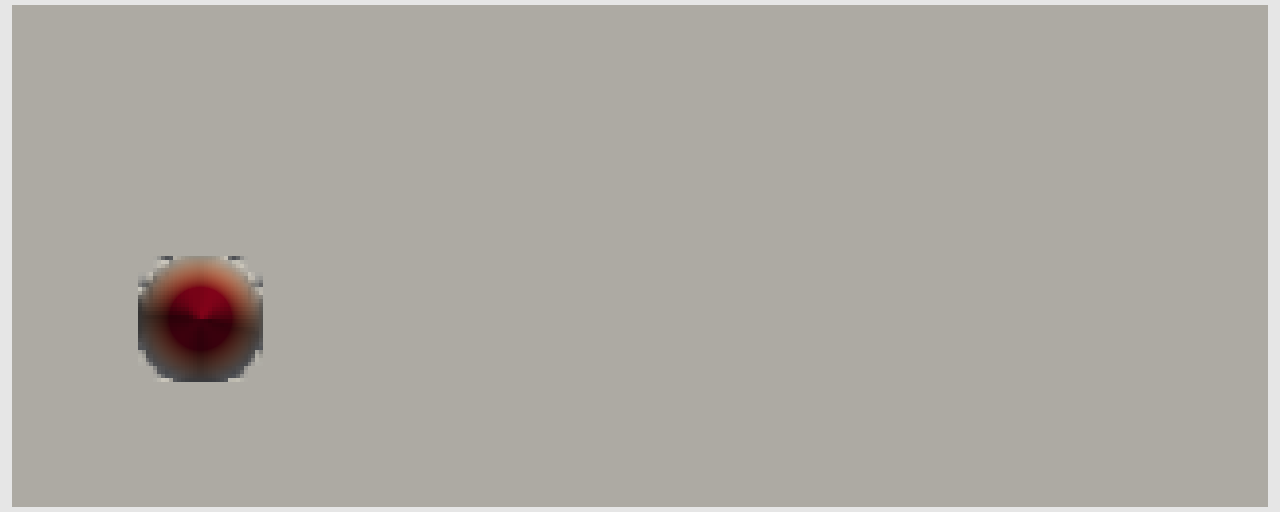
\includegraphics[width=0.499\textwidth]{wave_0}\hfill
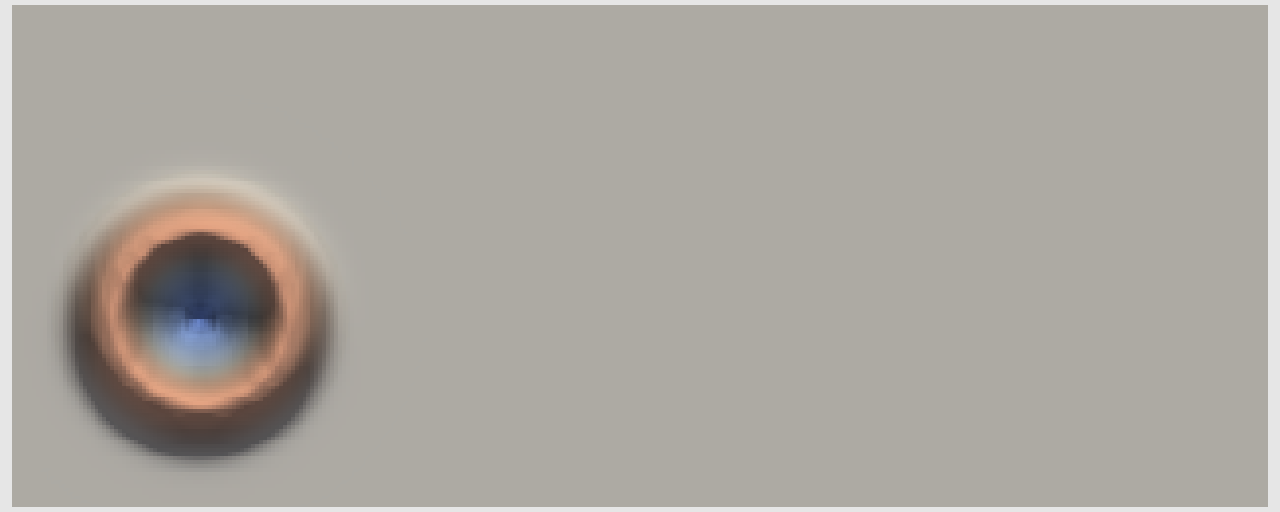
\includegraphics[width=0.499\textwidth]{wave_1}
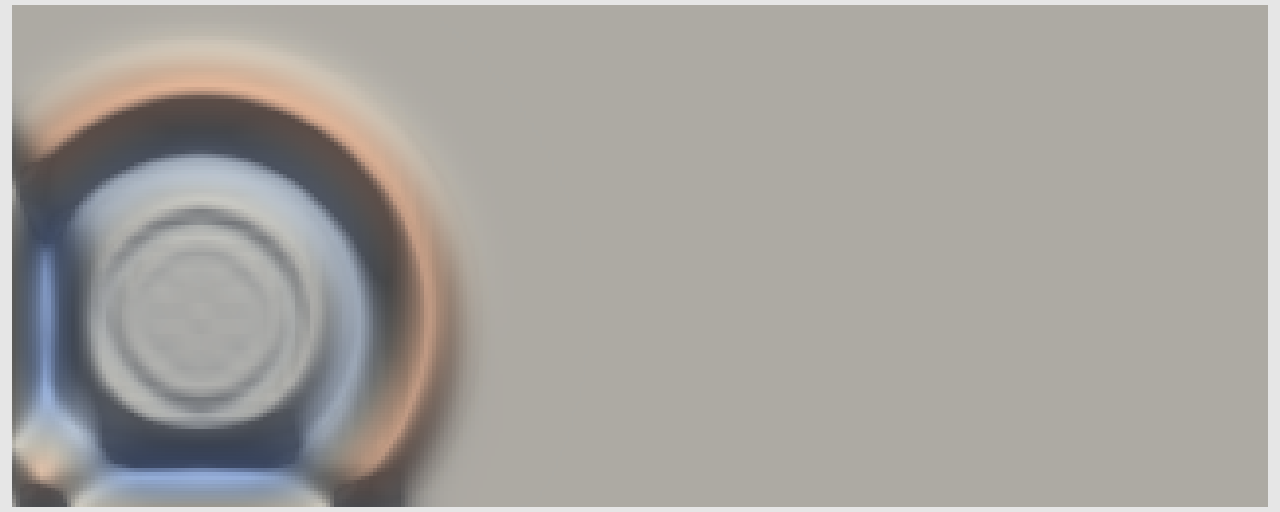
\includegraphics[width=0.499\textwidth]{wave_2}\hfill
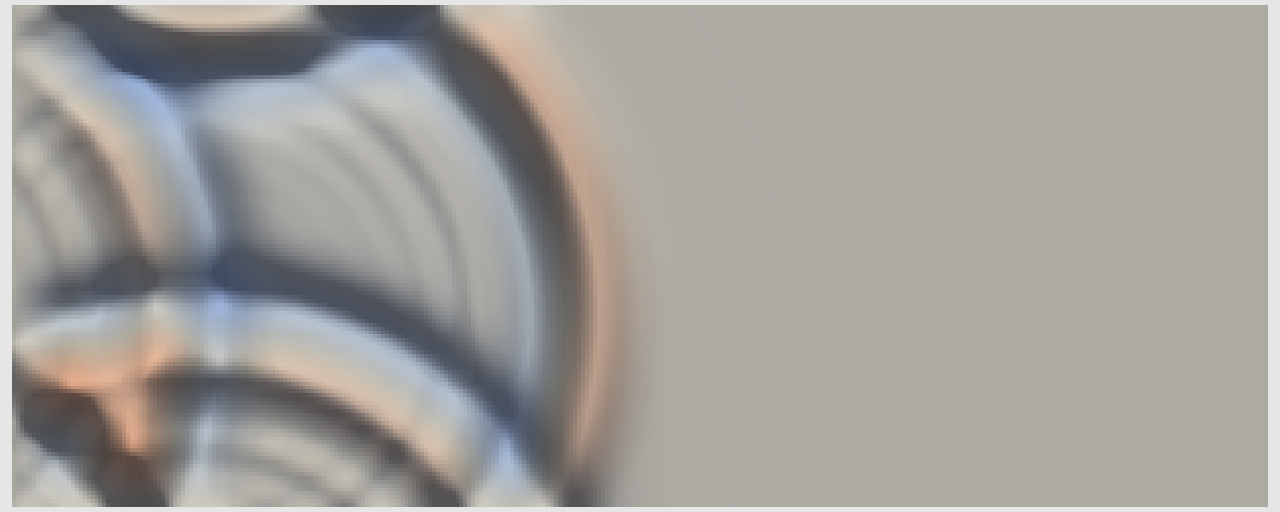
\includegraphics[width=0.499\textwidth]{wave_3}
\end{center}
\caption{Solution of the wave equation at four different times. Time is proceeding left
to right, top to bottom.}
\label{fig:Bunt}
\end{figure}

The example solves the wave equation in the domain
$\Omega = (0,2.5)\times (0,1)^{d-1}$ with a bump-like
initial condition. The results for the two-dimensional case are
illustrated in Figure \ref{fig:Bunt}. The initial bump has a height of 1
while the color code corresponds to blue for $-0.5$ and red for $0.5$.

\section{Outlook}

The following ideas could be explored from this tutorial:
\begin{itemize}
\item Explore polynomial degree greater than $2$ by changing the blocking
to \lstinline{none}.
\item Compute the total energy $E(t) = \|\partial_t u\|_{0,\Omega}^2 +
  \|\nabla u\|_{0,\Omega}^2$ and check its conservation in
the numerical scheme.
\item Try various time integrators, in particular the Crank-Nicolson method.
\item Implement the elliptic projection method of \cite{Eriksson} from
equation \eqref{eq:Eriksson}.
\end{itemize}

% bibtex bibliography
\bibliographystyle{plain}
\bibliography{tutorial04.bib}

\end{document}
